 \documentclass[a4paper]{article}
\author{Oscar Emil Sommer \\
A. Anand}
\makeatletter
\usepackage{amsfonts}
\usepackage{amsmath}
\usepackage{amssymb}
\usepackage{amsthm}
\usepackage{bm}
\usepackage[english]{babel}
\usepackage{booktabs}
\usepackage[margin = 10pt, font = small, labelfont = bf]{caption}
\usepackage{fancyhdr}
\usepackage{graphicx}
\usepackage{xcolor}
\usepackage{mathtools}
\usepackage{microtype}
\usepackage{multirow}
\usepackage{pdflscape}
\usepackage{pgfplots}
\usepackage{siunitx}
\usepackage{tabularx}
\usepackage{tikz}
\usepackage{sectsty}
\usepackage{derivative}
\usepackage{braket}
\usepackage[colorlinks=true
   ,urlcolor=blue
   ,anchorcolor=blue
   ,citecolor=blue
   ,filecolor=blue
   ,linkcolor=blue
   ,menucolor=blue
   ,linktocpage=true
   ,pdfa=true
]{hyperref}

\pagestyle{fancyplain}
\fancyhead[R]{Oscar Emil Sommer \\
A. Anand}
\fancyfoot{}
\fancyfoot[C]{\thepage}

\renewcommand{\@dotsep}{10000} %No dots in ToC
\allsectionsfont{\bfseries\sffamily} %Sections are bold sans serif



% Theorem-like environments
\theoremstyle{definition}
\newtheorem*{axiom}{Axiom}
\newtheorem*{aprx}{Approximation}
\newtheorem*{claim}{Claim}
\newtheorem{theorem}{Theorem}[section]
\newtheorem{corollary}[theorem]{Corollary}
\newtheorem{definition}{Definition}[section]
\newtheorem{conjecture}{Conjecture}
\newtheorem*{example}{Example}
\newtheorem*{exercise}{Exercise}
\newtheorem*{fact}{Fact}
\newtheorem*{remark}{Remark}
\newtheorem*{method}{Method}
\newtheorem{lemma}[theorem]{Lemma}
\newtheorem{proposition}[theorem]{Proposition}


\newtheorem*{principle}{Principle}
\setcounter{tocdepth}{2}
\makeatother

%Upright symbols
\renewcommand{\i}{\mathrm{i}}
\newcommand{\e}{\mathrm{e}}
\newcommand{\p}{\partial}
%Vector formatting
\renewcommand{\Vec}[2]{\left(\begin{array}{c} {#1} \\ {#2} \end{array}\right)}


%Common sets
\newcommand{\R}{\mathbb{R}}
\newcommand{\Z}{\mathbb{Z}}
\newcommand{\N}{\mathbb{N}}
\newcommand{\Q}{\mathbb{Q}}
\newcommand{\C}{\mathbb{C}}
\newcommand{\M}{\mathcal{M}}

%Common Groups
\newcommand{\SU}{\mathrm{SU}}
\newcommand{\SL}{\mathrm{SL}}
\newcommand{\GL}{\mathrm{GL}}
\newcommand{\Orth}{\mathrm{O}}
\newcommand{\SO}{\mathrm{SO}}
\newcommand{\U}{\mathrm{U}}
\renewcommand{\Im}{\operatorname{Im}}
\renewcommand{\Re}{\operatorname{Re}}


\newcommand{\su}{\mathfrak{su}}
\newcommand{\gl}{\mathfrak{gl}}
\newcommand{\so}{\mathfrak{so}}
%Common stylistic variable

\newcommand{\ep}{\epsilon}
\newcommand{\var}[1]{\delta #1\,}
\newcommand{\dd}[1]{\mathrm{d}#1\,}
\newcommand{\oes}[1]{\textcolor{red}{#1}}
\newcommand{\oesimp}[1]{\textcolor{blue}{#1}}
\newcommand{\vb}{\mathbf}
\newcommand{\ketbra}[2]{\ket{#1}\!\!\bra{#2}}
\newcommand{\Tr}{\operatorname{Tr}}
\newcommand{\up}{\uparrow}
\newcommand{\down}{\downarrow}


\fancyhead[L]{\textbf{Matrix product states}}


\begin{document}
\section{Lecture 1}
When investigating \emph{many-body quantum systems}, we generally want statistical properties,
even as our models are too complicated to solve exactly.

\begin{example}[Spin chain]
    A system of $L$ spins has a Hilbert space
    $\{\ket{\up},\ket{\down}\}^{\otimes L} $ 
    with  dimension $2^L$ making exact
    numerical calculations completely infeasible for $L\gtrsim 30$
    \begin{center}
    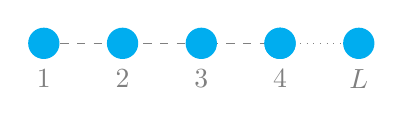
\begin{tikzpicture}
        \tikzset{bead/.style={circle,fill=cyan,inner sep=4pt}}
        \draw[dashed, gray] node[bead,label=below:$1$]{}(0,0)
            \foreach \spin in {2,...,4}
                { -- ++(1,0) node[bead,label=below:$\spin$]{}}
                edge[dotted] ++(1,0) node[bead]{} ++(1,0)
                node[bead,label=below:$L$]{};
    \end{tikzpicture}
    \end{center}
    
\end{example}
Instead we must change our mindset from finding information about all of the
states, and instead focus only on the relevant sectors. For most purposes the
states we are interested are near the \emph{ground state} or \emph{thermal
states}.  Hence we want a method to calculate states in these sectors, which is
where the matrix product state (MPS) method comes into play.\\
\begin{remark}[ MPS (\href{https://pitp.phas.ubc.ca/confs/sherbrooke2012/archives/PEPS.pdf}{PEPS}/TNS) methods] Key features are :
    \mbox{}
\begin{itemize}
    \item Works for 1D systems (For 2D, in developing phase yet!)
    \item Applicable for various system types like chains of bosons, fermions or spins (like Pott's chain etc)
    \item Works best for `low' entanglement states (quantified later)
    \item There is primarily a possibility of finding the ground state and the low energy excitations
    \item It is possible to find time evolution for both \emph{closed} and \emph{open} systems
    \item The method also works with finite temperature states
\end{itemize}
\end{remark}

\subsection{Idea of DMRG/MPS (Variational method)}
The matrix product state method is a variational method which relies heavily on
singular value decompositions (SVD) and the Schmidt decomposition.
\begin{method}[Singular Value decomposition]
    Any rectangular matrix $A$ of dimensions $(m\times n)$ can be decomposed as 
\[
A=USV^\dagger,
\]
where the matrices $U,S,V^\dagger$ are matrices with the below properties
\begin{description}
    \item[$U\,\,\,$:] A $\left(m\times\mathrm{min}(m,n)\right)$ matrix with $U^\dagger U=I$
    \item[$S\,\,\,$:] A $\left(\mathrm{min}(m,n)\times\mathrm{min}(m,n)\right)$ diagonal matrix with
            $S_{\alpha\alpha}=\sqrt{\lambda_\alpha}\geq0$
    \item[$V^\dagger$:] A $\left(\mathrm{min}(m,n)\times n\right)$ matrix with $V^\dagger V=I$
\end{description}
The rank of $S$ will turn out to be especially important and so in general we
will denote $r=\text{rank($S$)}$.
\end{method}
\begin{method}[Schmidt decomposition]
    Using SVD we can decompose a general element of a product space
    $\mathcal{H}_A\otimes \mathcal{H}_B$ from a double sum over tensor products
    of basis elements to a single sum over an orthonormal Schmidt basis as follows
\begin{align*}
\ket{\psi}&=\sum_{ij}\psi_{ij}\ket{i}_A\ket{j}_B\\
&= \sum_{ij\alpha}U_{i\alpha}\sqrt{\lambda_\alpha} V_{j\alpha}^*\ket{i}_A\ket{j}_B\\
&=\sum_{\alpha=1}^r \sqrt{\lambda_\alpha}\left(\sum_i U_{i\alpha}\ket{i}_A\right)\left(\sum_j
V_{j\alpha}^* \ket{j}_B\right)\\
&=\sum_{\alpha=1}^{r}\sqrt{\lambda_\alpha}\ket{\alpha}_A\ket{\alpha}_B\tag{$\star$}\label{eq:schmidtdecomp}
\end{align*}
\end{method}
The Schmidt decomposition is exact and the coefficients $\lambda_\alpha$ tell us very useful
information about what happens if we trace out one of the two subsystems. It
also provides the minimal number $r$ of coefficients by which we may describe
$\ket{\psi}$ using a product basis. 

\hrulefill

\noindent\textbf{Digression : $\rho$ after Schmidt decomp.}\\

\noindent Although, we lose the familiarity of product basis set $ \{ \ket{i}_A$, $\ket{j}_B \}$, what we gain is the
simplicity in the form of density matrix $\rho$. 
\begin{align*}
\rho &= \ket{\psi} \bra{\psi} \\
&= \sum_{ij}\sum_{kl} \psi^{*}_{kl} \psi_{ij} \ket{i}_{A}\ket{j}_{B} \bra{k}_{A} \bra{l}_{B}\\\
\text{after Schmidt decomp.} &= \sum_{\alpha,\beta=1}^r \sqrt{\lambda_\alpha\lambda_\beta}\ket{\alpha}_{A}\ket{\alpha}_{B} \bra{\beta}_{A} \bra{\beta}_{B} \\
\end{align*}

As we know, $\Tr \rho = 1$, that implies the singular values of this particular SVD follow $\sum_\alpha^{r} \lambda_\alpha = 1$.

\hrulefill
\vspace{0.5cm}

The point of matrix product states is now to find a way of implementing
a variational technique for the  states $\ket{\tilde{\psi}}$
which takes the form of \eqref{eq:schmidtdecomp} with only $D\leq r$ terms. The
point will be to vary the basis and coefficient to minimise
$||\ket{\tilde{\psi}}-\ket{\psi}||$.
Without loss of generality we may order the coefficients $\lambda_1\geq
\lambda_2\geq\dots \geq \lambda_r$, which allows us to calculate the minimal
distance
\[ 
\left\lVert\ket{\tilde{\psi}}-\ket{\psi}\right\rVert^2=1-\sum_{\alpha=1}^D \lambda_\alpha.
\]
It is therefore self-evident that this is good approximation if $\lambda_\alpha$ decay quickly.

\subsection{Quantifying validity of approximation}
By thinking of our total system as consisting of two subsystems, and tracing out
one of them we can illuminate the meaning of the coefficients.
\begin{center}
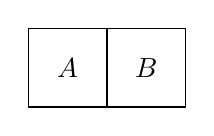
\begin{tikzpicture}
    \draw (0,0) -- (-1,0) -- (-1,1) -- (0,1) -- (0,0);
    \draw (0,0) -- (1,0) -- (1,1) --(0,1) -- (0,0);
    \draw (-0.5,0.5) node[] (){$A$} (0.5,0.5) node[](){$B$};
\end{tikzpicture}
\end{center}
Suppose we are in a pure state of the total system so that
$\rho=\ketbra{\psi}{\psi}$. The reduced density matrices for the subsystems may
be found by tracing out the other part of the Hilbert space 
\begin{align*}
\rho_A&=\Tr_B \rho,\\
\rho_B&=\Tr_A \rho.
\end{align*}
The coefficients $\lambda_\alpha$ are therefore the eigenvalues of the reduced density matrices.
A measure of how mixed the state is the von-Neumann entropy

\[S= - \Tr \rho_A\ln \rho_A=-\sum_\alpha \lambda_\alpha \ln \lambda_\alpha,\]


which is small when $\lambda_\alpha$ decay fast, and maximal when they are all
equal. Hence the approximation is good if $S$ is small.
\begin{remark}
From this we may conclude that MPS methods approximates the true state well for
low entropy states. An equivalent way of viewing these are as states with a low
amount of entanglement \emph{between the subsystems}\footnote{Ask lecturer to
clarify that it is the entanglement between two subsystems which is small}
\end{remark}
\begin{remark}
Some general theorems about the growth of entropy as system size increases are
known
\begin{itemize}
    \item  Ground state of 1D gapped system with short range interaction $S\to
    \mathrm{const}$ as $L\to \infty$. Hence we only require our approximate
    state to have rank $D\sim 2^\mathrm{const}$ indepedent of system size.\footnote{Shouldn't the
    ground state be a pure state? Ask follow up, if means ground state of
combined system $A+B$.}
    \item  Ground state of 1D critical system $S\to R \ln L+\mathrm{const}$ need $D\sim
        L^R$, which is polynomial in $L$, and therefore much more tractable than
        the exponential growth we see in the dimension of the full Hilbert
        space. 
\end{itemize}
\end{remark}
\subsection{What are MPS?}
So far we have no idea how we are going to implement our minimisation technique,
or where the matrix product states come into play. Any $\ket{\psi}\in
\mathcal{H}^{\otimes
L}$ state can be
decomposed into a so-called MPS by essentially unfolding the coefficients of
into a product of matrices. Let 
\[
\ket{\psi}=\sum_{\sigma_1\cdots\sigma_L} C_{\sigma_1,\dots,\sigma_L}\ket{\sigma_A}\otimes\cdots\otimes\ket{\sigma_L}
\]
be a representation of any given state. Now define a matrix $\psi$ of dim $d\times
d^{L-1}$ where $d=\mathrm{dim}\mathcal{H}$ by the relation
\[\psi_{\sigma_1,(\sigma_2,\dots,\sigma_L)}=C_{\sigma_1\sigma_2\dots\sigma_L}\]
Clearly we can do SVDs iteratively on $\psi$
\begin{align*}
    \psi_{\sigma_1,(\sigma_2,\dots\sigma_L)}&=\sum_{a_1=1}^{r_1} U_{\sigma_1,a_1}
S_{a_1,a_1} (V^\dagger)_{a_1,(\sigma_2,\dots,\sigma_L)}\\
&=\sum_{a_1=1}^{r_1} A^{\sigma_1}_{a_1} C_{a_1,\sigma_2,\dots \sigma_L}\\
&=\sum_{a_1=1}^{r_1}\sum_{a_2}^{r_2} A_{a_1}^{\sigma_1}
U_{(a_1,\sigma_2),a_2} S_{a_2a_2}
(V^{\dagger})_{a_2,(\sigma_3\dots\sigma_L)}\\
&=\sum_{a_1,a_2}
A_{a_1}^{\sigma_1}A_{a_1a_2}^{\sigma_2}\psi_{(a_2,\sigma_3)(\sigma_4\cdots)}\\
&=\sum_{a_1\dots a_{L-1}} A^{\sigma_1}_{a_1} A^{\sigma_2}_{a_1a2}\cdots
A_{a_{L-2}a_{L-1}}^{\sigma_{L-1}} A_{a_{L-1}}^{\sigma_L}
\end{align*}
Where we've decomposed the tensor coefficient into a product of matrices of
dimension  $(1\times d)(d\times d^2)\dots (d^{L/2-1} \times d^{L/2})( d^{L/2}
\times d^{L/2 -1})\dots(d\times 1)$. It can be nice to think about what we are
doing in diagrams, by representing a tensor as a square with lines corresponding
to each index. Our matrix product state then is constructed by pulling apart
each of the external indices as



\begin{center}

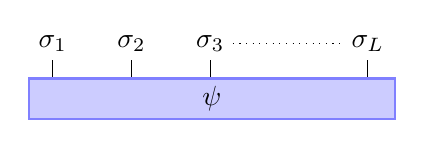
\begin{tikzpicture}[inner sep=1mm]
    \tikzstyle{tensor}=[rectangle,draw=blue!50,fill=blue!20,thick]
    \foreach \i in {1,...,3} {
        \node[tensor] (\i) at (\i, 0) {};

        \node[] (s\i) at (\i, 0.7) {$\sigma_\i$};
        \draw[-] (\i) -- (s\i);
    };

    \draw (3) edge[dashed] (5,0);
    \node[tensor](5)at (5,0){};
    \node (s5) at (5,0.7) {$\sigma_L$};
    \draw[-] (5) -- (s5);

    \draw[dotted] (s3) -- (s5);

    \node[tensor,minimum width=4.65cm] (0) at (3.02, 0) {$\psi$};
\end{tikzpicture}\\
{\large$\Downarrow$}\\
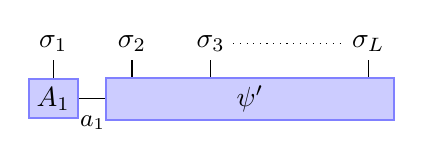
\begin{tikzpicture}[inner sep=1mm]
    \tikzstyle{tensor}=[rectangle,draw=blue!50,fill=blue!20,thick]
    \foreach \i in {1,...,3} {
        \node[tensor] (\i) at (\i, 0) {$A_\i$};

        \node[] (s\i) at (\i, 0.7) {$\sigma_\i$};
        \draw[-] (\i) -- (s\i);
    };

    \draw (3) edge[dashed] (5,0);
    \node[tensor](5)at (5,0){};
    \node (s5) at (5,0.7) {$\sigma_L$};
    \draw[-] (5) -- (s5);

    \draw[dotted] (s3) -- (s5);
    \draw[-] (1) edge[-]node[label=south:\small$a_1$]{} (2);
    \node[tensor,minimum width=3.65cm] (0) at (3.5, 0) {$\psi'$};
\end{tikzpicture}\\
{\Large$\Downarrow$}\\
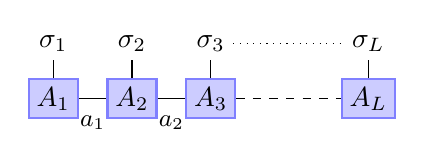
\begin{tikzpicture}[inner sep=1mm]
    \tikzstyle{tensor}=[rectangle,draw=blue!50,fill=blue!20,thick]
    \foreach \i in {1,...,3} {
        \node[tensor] (\i) at (\i, 0) {$A_\i$};
        \node (s\i) at (\i, 0.7) {$\sigma_\i$};
        \draw[-] (\i) -- (s\i);
    };
    \foreach \i in {1,...,2} {
        \pgfmathtruncatemacro{\iplusone}{\i + 1};
    \draw (\i) edge[-] node[label=south:\small$a_\i$]{}(\iplusone);
};

    \draw (3) edge[dashed] (5,0);
    \node[tensor](5)at (5,0){$A_L$};
    \node (s5) at (5,0.7) {$\sigma_L$};
    \draw[-] (5) -- (s5);
    \draw[dotted] (s3) -- (s5);
\end{tikzpicture}
\end{center}
%TODO  Rewatch end 
\end{document}
